\section{界面设计}

\subsection{界面设计总览}
人机界面设计围绕角色分工和任务链路展开，整体采用统一登录入口与分角色工作台的组织方式。用户完成身份认证后，不同角色分别进入建模工作台、分析工作台和后台治理工作台。三类界面在导航位置、提示样式、状态反馈和日志入口上保持一致，以降低切换成本；在信息分区、操作入口和主视觉区域上则根据角色任务进行差异化设计。

从视觉层次上看，界面顶层均包含系统标题、当前项目或工作空间名称、角色标识、通知入口和个人菜单。左侧区域承担导航和对象切换功能，中部区域承担主要内容展示，右侧区域承担参数、属性、执行状态或明细信息展示。这样的布局既能够保持三类工作台在交互结构上的一致性，又能为不同角色提供有针对性的主操作区。

本章所述界面形态已结合生成的参考图进行整理。参考图为基于系统功能描述生成的设计示意，其作用在于辅助说明页面布局、视觉层次和信息分区，不作为最终实现界面或前端像素标准。报告中的界面描述以这些参考图所体现的结构关系为依据，并进一步将其转化为可实现的界面组织说明。

\subsection{登录入口界面}
登录入口界面采用简洁的双栏或单卡片结构。页面上方居中显示系统名称“智能城市生成系统”和简要说明文字，下方放置账号、密码和身份验证输入区，登录按钮位于表单底部居中位置。若采用双栏布局，左侧可展示城市场景示意图、系统能力摘要或三维城市缩略背景，右侧放置登录卡片；若采用单卡片布局，登录框位于页面中央，背景采用淡色城市网格、道路纹理或简化天际线图案。

该页面的重点是形成清晰的进入路径，而不是承载复杂信息，因此交互元素保持精简。除基础登录控件外，页面只保留“记住登录状态”“忘记密码”或“联系管理员”等辅助入口。登录失败时在表单附近以醒目的提示条显示错误信息；登录成功后根据用户角色自动跳转到对应工作台。

图~\ref{fig:ui_login_reference} 所示的登录页参考图采用左右分栏结构，左侧以城市天际线和河道道路场景作为主视觉背景，并叠加系统名称、能力口号和三项核心能力摘要；右侧为白色登录面板，包含语言切换、账号密码输入、记住我、找回密码、主登录按钮以及单点登录、微信登录等辅助入口。该图清楚表达了系统在视觉上兼顾“城市场景特征”和“企业软件入口”的设计方向，适合作为登录页的表现参考。

\begin{figure}[!htbp]
\centering
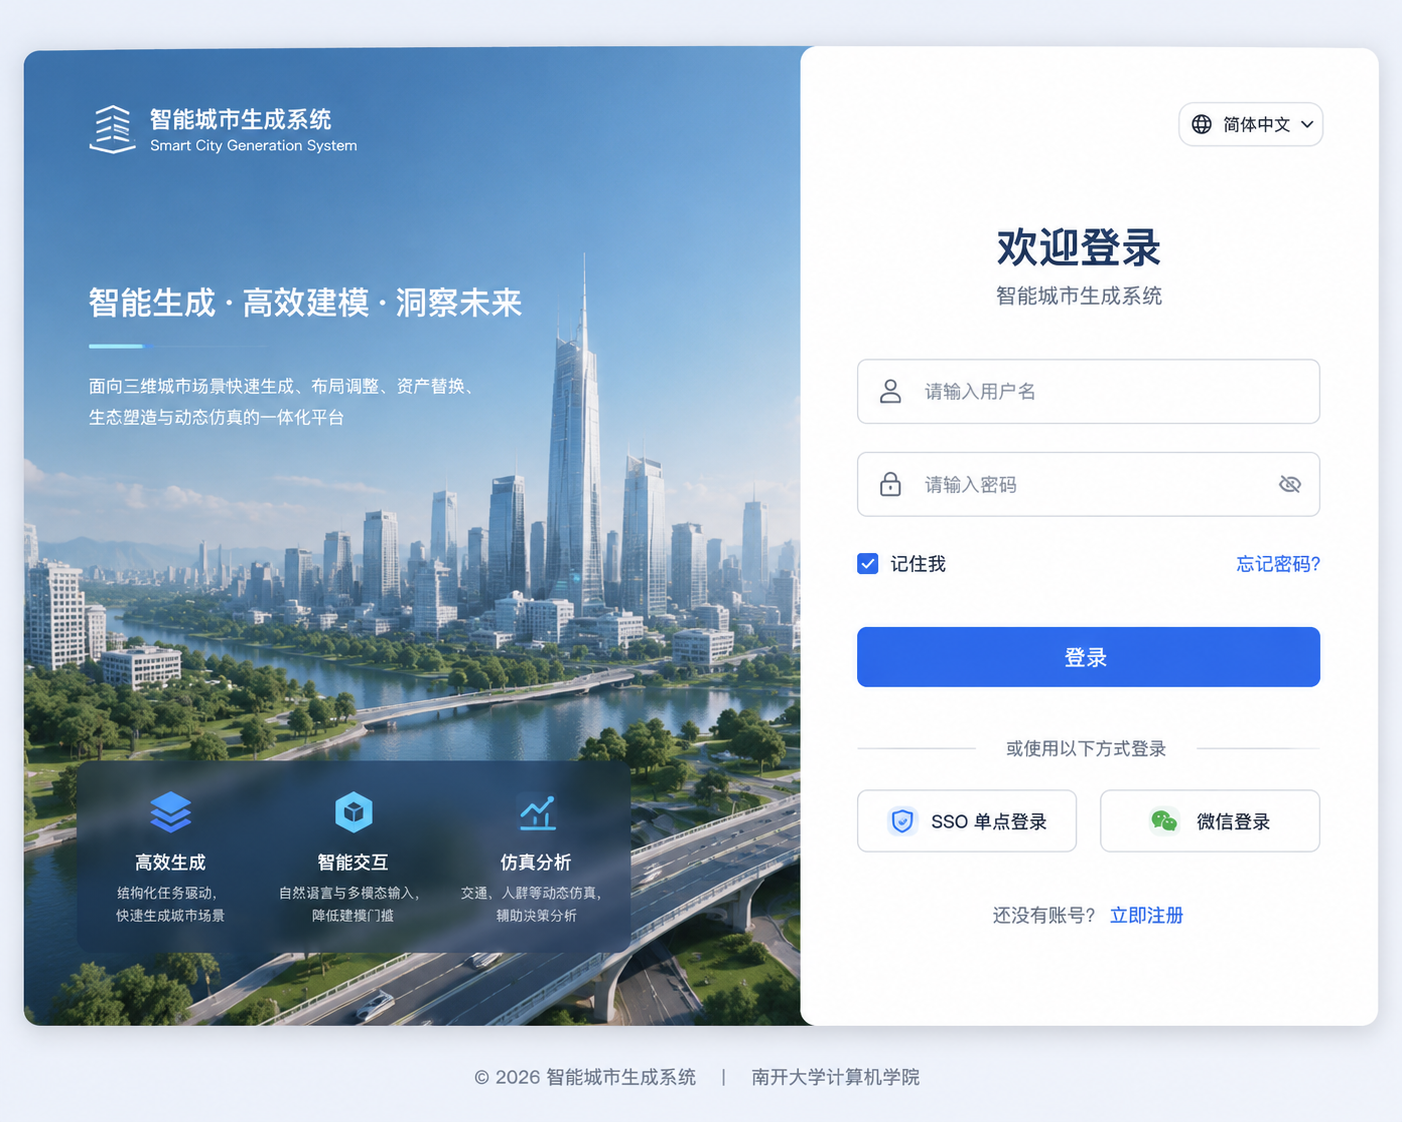
\includegraphics[width=\textwidth]{figures/11.png}
\caption{登录入口界面参考图}
\label{fig:ui_login_reference}
\end{figure}

\subsection{建模工作台}
建模工作台是系统的核心生产界面，整体采用三栏式结构。左栏用于项目与场景资源管理，顶部显示当前项目名称、版本号和最近保存时间，下方依次放置项目列表、场景版本树、资源分类标签以及可折叠的道路、建筑、植被、水体等资源面板。中部为主视图区，采用大尺寸三维场景预览窗口，可显示当前城市模型、控制点、布局轮廓和局部修改结果；主视图区下方放置时间轴、预览缩略条或版本对比切换入口。右栏为任务与参数区，按照“输入内容 - 结构化任务解释 - 参数确认 - 执行状态 - 结果摘要”的顺序自上而下排列。

在交互呈现上，建模师既可以通过文本输入框描述城市生成意图，也可以上传草图、点线集或参数模板。输入区下方显示系统生成的任务解释卡片，卡片内列出目标对象、数量、空间关系、限制条件和预计调用的插件能力。确认按钮、重新解析按钮和取消按钮位于任务卡片下方，执行后右栏切换为状态面板，显示排队中、执行中、成功或失败等状态标签、进度条和日志摘要。中部视图区在执行前后保持连续，便于建模师直接观察修改效果。

从界面氛围上看，建模工作台应突出“编辑中”的工作状态。中部三维视图占比最大，颜色以浅灰、蓝灰和少量强调色为主，资源列表和参数面板保持规整，执行按钮和异常提示使用高对比色进行区分。整体观感应接近专业设计软件或三维内容制作工具，而不是普通信息管理后台。

图~\ref{fig:ui_workbench_reference} 中的上左区域给出了建模工作台参考图，其结构与上述描述基本一致：左侧为导航与对象入口，中部为大尺寸三维城市视图，右侧为任务创建与任务状态区，下方额外保留任务队列表格。该设计强调“视图、任务、状态”三者在同一页面内联动，有利于支持文本输入、任务生成、结果观察和版本回看的连续操作。

\subsection{分析工作台}
分析工作台以结果查看、方案比较和仿真观察为中心，布局上可采用“左侧方案树 + 中央大视图 + 右侧指标面板”的结构。左栏显示项目、场景版本和分析方案列表，并支持切换不同时间片、不同策略或不同场景快照。中央区域是主要的结果展示窗口，可在静态城市视图、动态仿真回放视图和多方案分屏对比视图之间切换。右栏显示关键指标、统计图、筛选条件和导出入口，包括车辆密度、人流分布、船只流向、路网负载或区域热力强度等信息。

该界面不承担复杂建模编辑任务，因此输入控件明显少于建模工作台。顶部工具栏主要放置方案切换、回放控制、时间轴拖动、截图导出和报告生成按钮。中央主视图下方可配置仿真时间滑块、播放/暂停按钮和回放速度调节控件，用于观察动态变化。若采用双方案比较模式，中央区域可左右并排显示两个方案视图，中间保留同步滚动或联动回放开关。

在视觉表达上，分析工作台强调“观察”和“比较”。地图、三维场景、热力叠加层和动态图例构成主要视觉元素，图表和统计卡片辅助解释结果。界面应弱化资源库、参数编辑器和插件配置等生产型控件，使分析师能够将注意力集中在结果差异和指标变化上。

图~\ref{fig:ui_workbench_reference} 的上右区域展示了分析工作台参考图。该图采用热力覆盖与指标卡片并置的方式：中央显示带有交通与区域热力叠加效果的城市视图，右侧展示人口、交通、能耗等指标摘要及趋势图，下方提供图层控制和仿真对象筛选区。该布局较好地体现了分析界面对“结果读取、指标解释、方案对比”的侧重关系。

\subsection{管理员工作台}
管理员工作台采用信息管理后台样式，整体结构为“左侧功能导航 + 中央列表区域 + 右侧详情抽屉或下方详情面板”。左侧导航包含用户管理、角色权限、插件连接、模型服务、资源库状态、任务监控、日志审计和系统配置等模块。中央区域默认显示表格或卡片列表，支持搜索、筛选、排序和批量操作。右侧详情区在点击某一记录后展开，用于显示用户权限矩阵、插件状态明细、服务健康信息、错误日志片段或审计追踪记录。

管理员界面中的任务监控页应突出运行状态面板，上方放置服务健康概览卡片，例如“在线插件数”“任务排队数”“近一小时失败率”“模型服务响应时间”等摘要信息；下方显示任务列表和日志表格，每条记录包含任务编号、触发用户、当前状态、开始时间、结束时间和异常说明。权限管理页则更强调角色树、菜单矩阵和权限勾选区，以便管理员快速调整可见功能和操作范围。

该工作台在视觉上应保持克制和清晰。颜色以中性色为主，异常状态使用橙色或红色强调，成功状态使用绿色标识。界面重点在于信息可检索、状态可定位、操作可追溯，不需要突出三维效果或沉浸式展示。

图~\ref{fig:ui_workbench_reference} 的下方区域给出了管理员工作台参考图。该图采用典型后台布局，上方为系统概览卡片，中部为趋势图与资源监控图，下方为项目存储使用情况、系统服务状态和最近日志列表。该图将管理员最关心的统计信息、运行状态和审计记录集中在同一页面上，适合作为后台首页或综合监控页的设计参考。

\begin{figure}[!htbp]
\centering
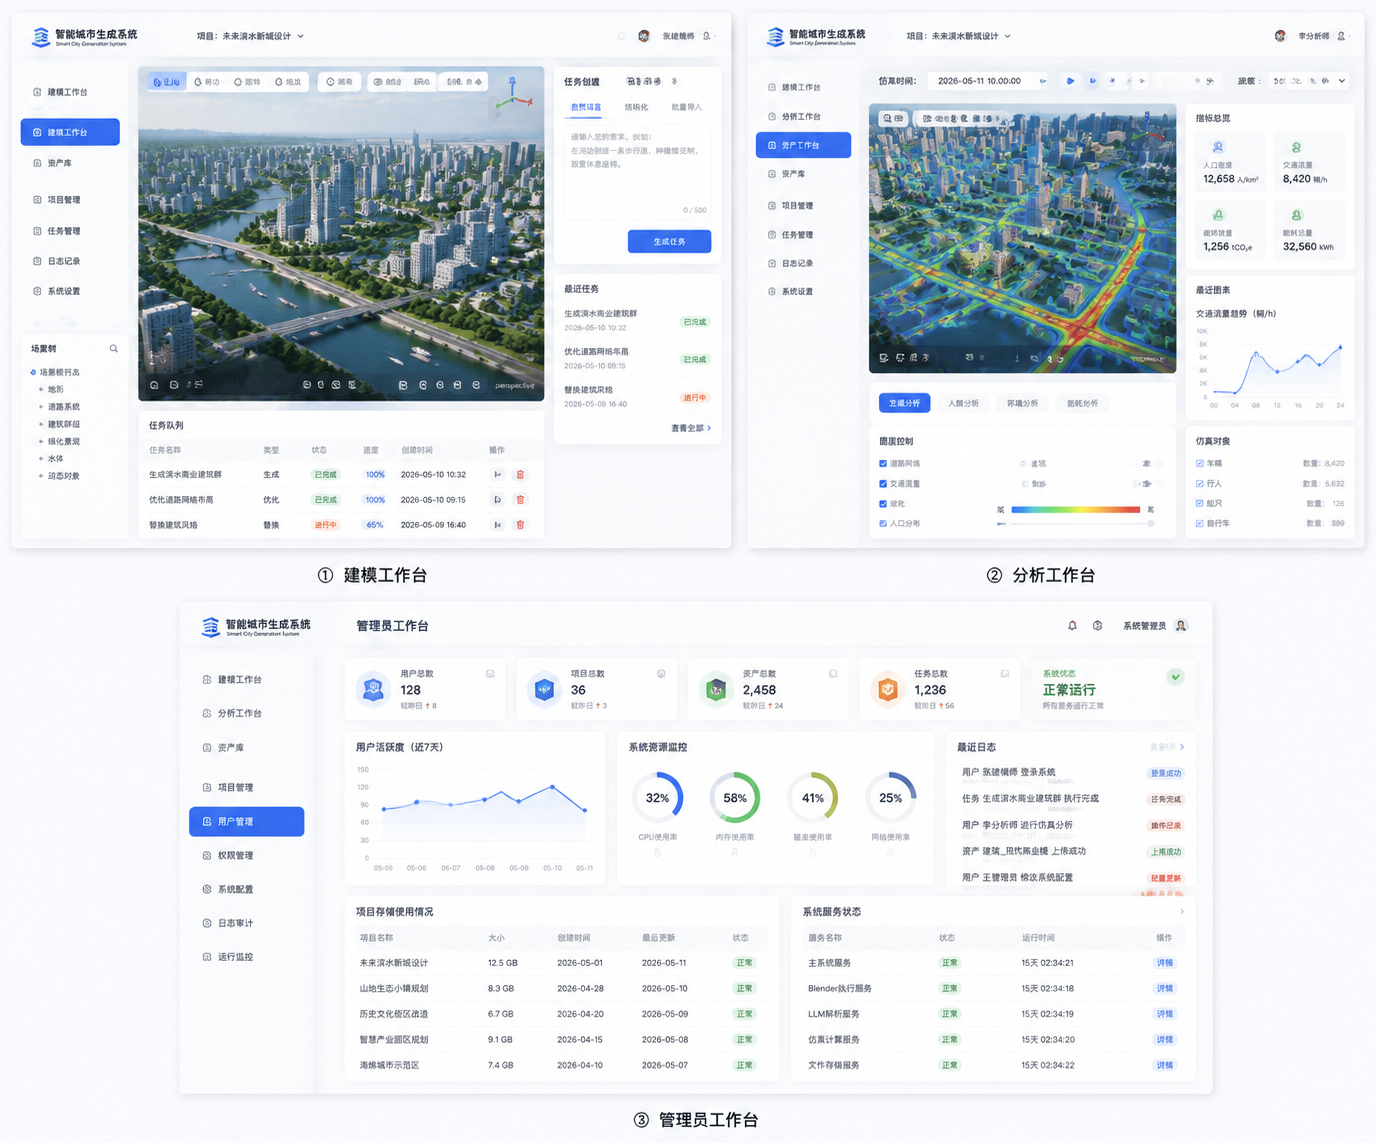
\includegraphics[width=\textwidth]{figures/12.png}
\caption{三类工作台界面参考图}
\label{fig:ui_workbench_reference}
\end{figure}

\subsection{界面设计原则}
\begin{enumerate}[label=\arabic*.]
    \item 执行前信息可解释：建模相关界面必须在任务下发前显示结构化解释、约束条件和关键参数。
    \item 状态反馈持续可见：排队、执行、成功、失败和回写等状态均需在显著位置连续显示。
    \item 角色入口保持收敛：每类角色仅暴露完成本职任务所需的主要功能和信息面板。
    \item 结果与版本易于回看：项目版本、仿真结果、日志摘要和导出入口应能快速定位。
    \item 主操作区视觉突出：建模工作台突出三维视图，分析工作台突出结果对比，管理员工作台突出列表与状态面板。
\end{enumerate}
